\chapter{Special Topic: Aspects of Programming}\label{ap:oop}

The focus of these research notes is on LFT, which employs programming heavily.
In particular the computationally demanding MCMC code we write spurs us to
write code that is
\begin{enumerate}
  \item easy to read,
  \item well organized,
  \item future-proof, and
  \item high performance.
\end{enumerate}
Furthermore we must carry out statistical analysis of observables measured on
configurations produced by this MCMC code. In this Appendix we collect
some information on these topics.


\section{Object oriented programming}


The first programming language I used for serious scientific calculations
\index{object-oriented programming}
was Fortran. Fortran does not traditionally 
allow\footnote{Actually I think more modern Fortran compilers 
allow for OOP, but I get the impression that C++ is the preferred language
in scientific computing for this.} for object-oriented programming (OOP); 
instead, very roughly, Fortran only
allows for two things:
\begin{enumerate}
  \item arrays or variables of some kind, along with 
  \item some functions that map them into each other.
\end{enumerate}
Actually programming in Fortran is kind
of a physicist's dream: it is very direct, and you can see exactly what
operations the computer is going to carry out. I will call Fortran
a {\it non-OOP} language.

An OOP language is more general than this, and hence it is a bit more powerful.
\index{compile-time}\index{runtime}
For the following discussion, it is useful to introduce two terms,
{\it compile-time}, which is the time during which the code you wrote
is turned into an executable, and {\it runtime}, which is the time during
which the executable runs.
Again very roughly, an OOP language has instead three things:
\begin{enumerate}\index{object}\index{function!OOP}\index{method}\index{class}
  \item {\it objects}, which I will define as any runtime entity that 
        takes up memory and has an address;
  \item {\it functions} or {\it methods}, which map objects to other
        objects; and
  \item {\it classes}, which are an abstraction of objects and/or functions,
        that do not take any space in memory or have an address.
\end{enumerate}

Ultimately an important goal of OOP is to try to make your code more closely
mirror how things look in the real world, and maybe you can see that this
goal is more readily accomplished under this paradigm.
For example in point (1), you can see that variables
and arrays were generalized to objects. This gives you more flexibility in
coding, in case the real-world object you are thinking of is not easily
imagined as a variable or an array. The way that we invent these objects
is through point (3), the class. In addition to defining objects, the
class is an important organizational tool, allowing you to collect all
objects and functions that are related to some general idea,
which\index{encapsulation}\index{abstraction} is sometimes called 
{\it encapsulation}. Both functions and classes
are useful to hide implementation details from the programmer, minimizing
the what the programmer needs to provide to the program, which is
sometimes called {\it abstraction}.

Encapsulation and abstraction are useful to programmers in part because
they make the code much more readable (again because what you are typing
more closely resembles how you think of things in the real world) and
reduce code duplication (which prevents you from having to maintain
several duplicates). Furthermore you
can change the implementation details of that class
without having to modify anything that utilizes it. The drawback is that
it can be difficult to see precisely what operations the computer
performs. In my experience, this trade-off is hugely worthwhile, and I think
most modern software developers would agree.

\subsection{OOP in C++} 
Probably the best way to learn is through an example. To see the basics
of OOP in action, we will implement a \texttt{CAT} class, and 
introduce some new OOP jargon and concepts along the way.
The example code definitely works for C++14~\cite{cppDocumentation},
but it likely also works for earlier standards.

The first function we define, \texttt{narrate}, is not part of the class;
actually it is there to make it easier to print to screen, which is
an example of abstraction. We see that it made the code easier to
read and reduced duplication.\\

\lstinputlisting[firstline=1,lastline=41]{exampleCode/cat.cpp}

The \texttt{CAT} class begins with the \texttt{public} keyword, which
is a statement about accessibility. Anything that falls under the
\texttt{public} heading can be used outside of the class\footnote{Another
possibility is \texttt{private}. Anything under the \texttt{private} heading
can only be seen by the class itself.}. Everything in the class falls
under this heading in this example. The first group of three lines
are variables stored inside the \texttt{CAT} class; such variables
\index{attribute}\index{constructor}\index{destructor}\index{method}
are called {\it attributes}. The next group of two functions are
the {\it constructor} and the {\it destructor}, which I will explain
shortly. Finally the last group of four \texttt{void} functions are 
called {\it methods}. It is basically correct to think of a class as a
collection of attributes and methods acting on them.\\

\lstinputlisting[firstline=42, lastline=54]{exampleCode/cat.cpp}

To understand the constructor and destructor, let us turn to our main
code where we will use this class. In the first line, we declare a
\texttt{CAT}-type object, which we call \texttt{cat}. We say that we have
{\it instantiated} \texttt{cat}, and \texttt{cat} is an {\it instance}
\index{instantiation}
of \texttt{CAT}. \texttt{CAT} is a class; therefore, as mentioned
earlier, it takes up no memory and has no address associated to it.
On the other hand, \texttt{cat} is an object, and hence has some
memory associated to it at runtime. More precisely, it uses the
amount of memory required to hold its attributes.

The constructor is the function that is called every time an object is
instantiated. If you look back at the \texttt{CAT} class, you can see that
the constructor takes an argument called \texttt{name}. In the main,
the string ``Chooky" is being fed into this argument. A constructor does
not have to take an argument, or even explicitly do anything, but often
it is useful to have a constructor set the attributes to some default values.
That is what the constructor does in this case, and it also tells the
user that it instantiated a \texttt{CAT} object.\\

\lstinputlisting[language={}]{exampleCode/catOutput.txt}

The destructor is the function called every time an object is destroyed.
The two most common times an object is destroyed are when the object
leaves scope and when the program ends. Scopes in C++ are defined by
curly brackets $\{\}$. So for example if you define a new variable
inside a function, and you only use this variable inside that function,
the {\it scope} of that variable is the inside of the function. 
Other examples of scope include
the inside of \texttt{if} and \texttt{while} statements and the
\index{scope}
insides of classes. Look to \texttt{scope.cpp} to see constructors and
destructors in action. Note the order of creation and destruction.

Turning back to the main, we see that we can access attributes of
\texttt{cat} such as \texttt{\_name} directly, and we can also call
methods of \texttt{cat} like \texttt{speak()}. This is possible because
we made these public attributes and methods. Note that inside the class,
it is enough to use the attribute or method name by itself. Outside the
class, i.e. inside the main, we have to use the object as an 
intermediary.

Hopefully this is enough for you to get at least an intuition for
what OOP is, how it works, and why someone would want to use it. These
few pages are just the beginning; there are many more advanced
features available to C++ that make classes extremely generalizable.
Besides the advantages of being object-oriented, C++ also has many
features that make it valuable for high-performance computing.
For example you can manipulate exactly where and how objects
are stored in memory. There are lots of good references for OOP
in C++ out there, but a good start might be Ref.~\cite{tp:cpp}.\\

\lstinputlisting[firstline=40, lastline=49]{exampleCode/scope.cpp}
\lstinputlisting[language={}]{exampleCode/scopeOutput.txt}

\subsection{OOP in Python}

We continue by discussing OOP in Python. Python is a rather friendly language
and it is popular for scientific programming, so you can find lots of useful
tutorials online, for instance here~\cite{pythonOOP}. We will use
Python3~\cite{python3}.

In this section we will demonstrate
a couple other important features of the OOP paradigm. In particular we will
discuss {\it inheritance},\index{inheritance} the process by which a
class (the {\it child}\index{child} class) inherits attributes and methods
from a more general class (the {\it parent}),\index{parent} and
{\it operator overloading}, \index{operator overloading} where one generalizes 
operators such as $+$ to function with objects of the class you defined.
Inheritance is useful organizationally as it helps you think of some class
as a special case of a more general class. Furthermore it reduces code
repetition, since the child has access to all methods and attributes defined in
the parent. Operator overloading enhances readability, for example by
helping your code more closely mirror mathematical notation.\\

\lstinputlisting[language=Python,firstline=1,lastline=31]{exampleCode/cat.py}

Let us begin by implementing the \texttt{CAT} class from before in Python,
which is shown in \texttt{cat.py}. One nice feature of Python classes
is the \texttt{\_\_doc\_\_} attribute, which is set here as the first string
in quotes, giving a description of the class. Note also that Python
does not have the \texttt{private} or \texttt{public} distinction that
C++ has; indeed all attributes and methods in Python OOP are effectively 
public\footnote{You can obfuscate attributes by leading with a double 
underscore \texttt{\_\_} so that it is not as easily accessible. Still, there 
are ways to access such attributes.}.
The constructor and destructor\footnote{Python does not treat scope the same
way as C++, so an object is not destroyed automatically when you e.g.
exit a \texttt{for} loop. Automatic object destruction in Python 
happens through \index{garbage collection}
its {\it garbage collector}, for example when the program terminates,
or when an object loses its reference by being reassigned.} are identified with
\texttt{\_\_init\_\_} and \texttt{\_\_del\_\_}, respectively. All of
\texttt{\_\_init\_\_}, \texttt{\_\_del\_\_}, and \texttt{\_\_doc\_\_} 
are examples of
Python special functions, which will be discussed in a bit more detail
when we get to operator overloading. 
Two more syntactical characteristics 
to point out are that methods always take the \texttt{self}\footnote{The
\texttt{self} keyword refers to particular instance which is using
the called method.} reference as 
the first argument, and that this reference is always required to
interact with class methods and attributes, even within the class itself.
Some example output code using the \texttt{CAT} class is shown below.\\

\lstinputlisting[language=Python,firstline=44,lastline=55]{exampleCode/cat.py}
\lstinputlisting[language={}]{exampleCode/pythonCatOutput.txt}

To demonstrate inheritance, we consider a new kind of \texttt{CAT}, a
\texttt{MEANCAT}. \texttt{MEANCAT}s prefer to hiss rather than meow, and
their \texttt{speak()} method should reflect this behavior. Nothing else
about a \texttt{MEANCAT} is different. To indicate that \texttt{MEANCAT}
should inherit from \texttt{CAT}, one just passes \texttt{CAT} as an argument
in the class definition\footnote{It is also possible for a class to inherit
from more than one parent. This is called {\it multiple inheritance},
\index{inheritance!multiple} and it can be accomplished in Python by passing
multiple arguments to the definition, e.g. \texttt{MEANCAT(CAT,MAMMAL)}.}. 
The redefinition of the \texttt{speak()} method
in \texttt{MEANCAT} overrides that of its parent, \texttt{CAT}. One last
feature to point out is the use of the \texttt{del} keyword, which lets you
call an object's destructor.\\

\lstinputlisting[language=Python,firstline=32,lastline=41]{exampleCode/cat.py}
\lstinputlisting[language=Python,firstline=56,lastline=66]{exampleCode/cat.py}
\lstinputlisting[language={}]{exampleCode/meanCatOutput.txt}

Finally we will have a look at operator overloading. For this example we
will create a (rudimentary and wildly incomplete) class for a simple math 
object of interest to high energy physics: the $\SU(2)$ matrix.\\

\lstinputlisting[language=Python,firstline=1,lastline=42]{exampleCode/SU2.py}

Here the attributes are the elements of the matrix. 
I have opted to use double underscores \texttt{\_\_} in front of
the attribute names. As mentioned in an earlier footnote, this hides the
attributes from the user as shown below.
Hiding these attributes is important for the \texttt{SU2} class, because the
elements should always be \texttt{complex}, and I want to make sure the
user cannot accidentally change the type. The \texttt{complex} type is
enforced here through the \texttt{setElement} method.

\lstinputlisting[language=Python,firstline=53,lastline=55]{exampleCode/SU2.py}
\lstinputlisting[language={},firstline=5,lastline=8]{exampleCode/SU2Output.txt}

To use operator overloading, each binary operator has a special function name.
In the \texttt{SU2} class example, we overloaded the + operator. Its special
function name is \texttt{\_\_add\_\_}, and the two arguments are the LHS and
RHS of the operator, respectively. Python allows also for the overloading
of other algebraic operators, bitwise operations, and comparison operators.
In our example, we have edited the \texttt{\_\_str\_\_} operator, which
controls how an \texttt{SU2} object is printed to screen.

Below we give some quick examples of this \texttt{SU2} class in use. Note that
the = sign here is not a copy constructor; instead both \texttt{g} and
\texttt{h} are references to the same \texttt{SU2} object. This means that
if you change \texttt{g}, \texttt{h} will change as well. Be careful!\\ 

\lstinputlisting[language=Python,firstline=46,lastline=52]{exampleCode/SU2.py}
\lstinputlisting[language={},firstline=1,lastline=4]{exampleCode/SU2Output.txt}


\section{Dealing with binary files}

\index{binary}\index{binary!file}
The configurations that we generate store lots of information, and to make a
file human-readable costs extra storage space. Hence we must store
configurations as binary, to save space. Unfortunately\footnote{I feel your
pain, and I wish I could hug you right now. I'm so, so sorry.} for you,
this means you will have to learn in detail how a computer reads and writes data
to a machine.

\index{bit}\index{byte}
We start with the basics. A {\it bit} is the smallest unit of data a computer
can process or store. Each bit is represented as a 0 (false) or 1 (true).
Eight adjacent bits are organized into a {\it byte}.
Since the fundamental information unit has two possibilities, storage
sizes must exist in powers of two. For this reason, the naming scheme
for larger numbers of bytes is collected in powers of $2^{10}=1024$
instead of 1000 like it usually goes with the metric system.
In \tabref{tab:byte} we collect the tower of storage sizes
along with some references to get a feeling for how much information
they store. This whole two-bit numbering system is, as you probably
already know, called {\it binary}.

\index{byte!peta}
\index{byte!exa}
\index{byte!zetta}
\begin{table}
\centering
\caption{Converting bits to bytes.}
\begin{tabularx}{\linewidth}{lCLr}
\hline\hline
Name & Abbreviation & Bits & Information of...\\
\hline
kilobyte & KB & $1024$ & page of text \\
megabyte & MB & $1024^2$ & pop song MP3 \\
gigabyte & GB & $1024^3$ & computer game \\
terabyte & TB & $1024^4$ & laptop's storage \\
petabyte & PB & $1024^5$ & library of congress \\
exabyte  & EB & $1024^6$ & Google's storage capacity \\
zettabyte  & ZB & $1024^7$ & all data on internet \\
\hline\hline
\end{tabularx}
\label{tab:byte}
\end{table}

\index{hexadecimal}
Besides the binary numbering system another common system organizes things in
base 16. This is the {\it hexadecimal} system. Since we have only ten numerals,
this requires the introduction of some letters for its representation,
as shown in \tabref{tab:hexadecimal}. In C and C++ programming,
hexadecimal numbers are preceded by an indentifier \texttt{0x} to
indicate that it's hexadecimal\footnote{Instead it is preceded
by \texttt{0b} if it's binary.}.
Since hexadecimal is base 16, it follows that each hex digit is equivalent
to four bits. Hence the length of a hexadecimal number in C and C++
depends on the size of the object it represents. Finally, sometimes
a hexadecimal can be appended with a string like \texttt{ull} to
indicate it represents an \texttt{unsigned long long} object. 

\begin{table}
\centering
\caption{Converting decimal to hexadecimal.}
\begin{tabularx}{\linewidth}{CCCCCCCCCCCCCCCC}
\hline\hline
0 & 1 & 2 & 3 & 4 & 5 & 6 & 7 & 8 & 9 & 10 & 11 & 12 & 13 & 14 & 15\\
0 & 1 & 2 & 3 & 4 & 5 & 6 & 7 & 8 & 9 & a & b & c & d & e & f\\
\hline\hline
\end{tabularx}
\label{tab:hexadecimal}
\end{table}

In any such numbering system, numbers are represented with the least significant
digit in the right-most place. For example one has for decimal, binary, and
hexadecimal, respectively
\begin{equation*}\begin{aligned}
  \texttt{11} &= 1\times10^1+1\times10^0, \\
  \texttt{101} &= 1\times2^2+0\times2^1+1\times2^0,~\text{and} \\
  \texttt{0xf0} &= 15\times16^1+0\times16^0.
\end{aligned}\end{equation*}
While this is the way humans read significant digits, how the computer stores
binary depends on a convention called the {\it endianness}.
The storage is {\it big endian} \index{endian!big} if the most significant digit 
is at the smallest memory address. Conversely the
{\it little endian} \index{endian!little} convention specifies the least
significant digit is at the smallest memory address\footnote{I guess the way
to remember this is whether the smallest memory address starts at the most
significant digit, i.e. the big end, or the other way around.}.

\index{bit!mask}
Sometimes you may encounter {\it bit masking}. The idea is that one compares
two binary numbers bit-by-bit, and new binary is created by a logical operator
applied to each bit. For example
\begin{equation*}
  \texttt{001 \& 111} = \texttt{001}. 
\end{equation*}


\section{Evaluating performance}

Lattice projects are extremely computationally demanding; for instance
a recent HotQCD study utilized ensembles that required
$\order{2000}$ GPU-years of compute time and take up 2.4 PB of storage 
space~\cite{Bollweg:2021vqf}. Meeting this computational demands is
not cheap, so it is crucially important that your code is highly
optimized to get the most bang for your buck.
In this section we'll review some key concepts and terminology
relevant to assessing the performance of code
in high-performance computing (HPC). 

In this context, it is useful to define a few terms. A floating
point operation\index{FLOP} is a calculation of floating point arithmetic. In a
scientific context, this type is very common, so FLOPs are a good indicator
of the amount of arithmetic a code is doing. Any scientific code you write will
be in effect processing data. The rate at which data is processed
is called the {\it throughput},\index{throughput} 
and it can be measured in, for instance, FLOPs
per second, sometimes indicated\footnote{Please take care not to
mix up FLOPs with FLOP/s.} FLOP/s. The rate at which data is
transferred is called the {\it bandwidth},\index{bandwidth}
which can be measured in bytes/s.

\begin{figure}[t]
  \centering
  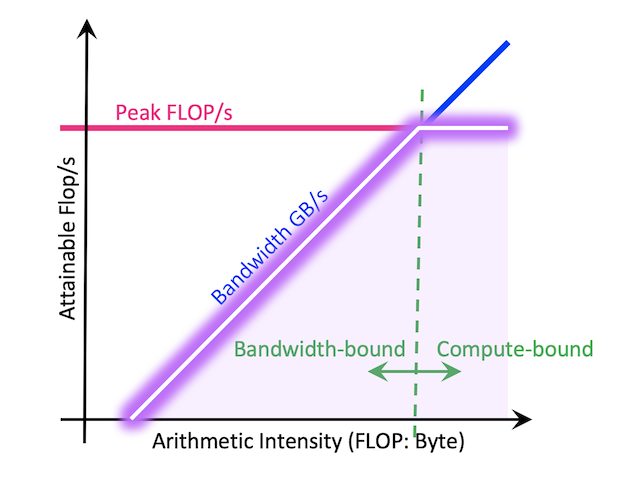
\includegraphics[width=\linewidth]{figs/Roofline-intro.png}
  \caption{Schematic example of a roofline analysis.
           Image taken from Ref.~\cite{roofline}.
           The light purple line indicates the theoretical
           maximum performance under this model.}
  \label{fig:roofline}
\end{figure}


\subsection{Roofline performance model}
\index{roofline performance analysis}


Obviously performance is limited by the hardware carrying out a calculation, for
instance the CPU, but it is also limited by the rate at which things are loaded
and extracted from memory. The {\it roofline performance model} is an elementary
way to see where your code stands with respect to these two limitations.

The {\it arithmetic intensity}\index{arithmetic intensity} of some code is
\begin{equation}
  \text{AI}=\frac{\text{\# FLOPs}}{\text{data movement in bytes}},
\end{equation}
where the numerator represents the number of FLOPs needed by that code, and the
denominator represents how much data you need to move in bytes in order to
support those FLOPs. From this equation it's clear that the attainable
FLOP/s scales linearly with arithmetic intensity.

Fig.~\ref{fig:roofline} shows a sketch of this model. The vertical
dashed line gives the {\it machine balance point}.\index{machine balance point}
This analysis is useful to try to diagnose whether one should look into
memory efficiency or algorithm improvement to try to speed up the code.
Code in the purple region to the left of the machine balance point
tends to be limited by bandwidth.


\bibliographystyle{unsrtnat}
\bibliography{bibliography}

